\documentclass{beamer}
\usetheme{metropolis}
\usepackage{graphicx}
\usepackage{boolexpr}
\usepackage{kpfonts}
\usepackage{caption}
\usepackage{wrapfig}
\usepackage{tkz-graph}
\usepackage{tikz}
\usepackage[labelformat=empty]{caption}
\usepackage[official]{eurosym}

\usepackage{siunitx}

\usepackage[math]{iwona}
\usepackage{scalerel}
\def\lVert{\mid\!\mid}
\def\rVert{\mid\!\mid}

\usepackage[normalem]{ulem}
\usepackage{mathtools}

\usepackage{custom}
\usepackage{amsfonts}
\newcommand{\jsrcodepath}{../../code}
\usepackage{jsr}

\newcommand{\expe}[2]{\la #1, #2 \ra}

\usepackage{framed}

\newcommand\Wider[2][3em]{%
\makebox[\linewidth][c]{%
  \begin{minipage}{\dimexpr\textwidth+#1\relax}
  \raggedright#2
  \end{minipage}%
  }%
}

\newcommand{\aeur}{\alpha_\text{\euro}}
\newcommand{\adol}{\alpha_\$}
\newcommand{\apou}{\alpha_\text{\pounds}}

\newcommand{\cssystemtikz}[2]{
  \begin{center}
    \begin{tikzpicture}[x=#1,y=#2]
      \Vertex{1}
      \NO[unit=4](1){2}
      \SOEA[unit=2](2){3}
      \EA[unit=2](3){4}
      \tikzset{EdgeStyle/.style = {->}}
      \tikzset{LoopStyle/.style = {->}}
      \tikzset{EdgeStyle/.append style = {bend right=18}}
      \Edge[label=1](1)(3)
      \Edge[label=3](1)(2)
      \Edge[label=2](2)(1)
      \Edge[label=1](2)(3)
      \Edge[label=2](3)(1)
      \Edge[label=3](3)(2)
      \Edge[label=4](3)(4)
      \draw[thick,->] (3) to [out=115,in=65,looseness=20] node [midway, fill=white] {1} (3);
      \Edge[label=1](4)(3)
    \end{tikzpicture}
  \end{center}
}

\title{Certifying unstability of Switched Systems using Sum of Squares Programming}
\date{}
\author{Beno\^it Legat (UCL), Rapha\"el M. Jungers (UCL) and Pablo A. Parrilo (MIT)}
\institute{Institute of Information and Communication Technologies, Electronics and Applied Mathematics (ICTEAM),\\
           Universit\'e catholique de Louvain (UCL)\\
           Laboratory for Information \& Decision Systems (LIDS)\\
           Massachusetts Institute of Technology (MIT)\\\\}

\makeatletter
\let\@@magyar@captionfix\relax
\makeatother

\begin{document}
  \maketitle
  \begin{frame}
      \frametitle{Motivating application}
      \begin{center}
          Simulation error
          \hspace{0.98em}
          $\Longleftrightarrow$%
          \hspace{1em}
          Dynamical system\footnote{Based on joint work with Cl\'audio Gomes from the University of Antwerp}
          \hspace{1em}
      \end{center}
      \[ \dot{x} = Ax \]
      \begin{center}
          \fbox{\parbox[m][9em][t]{0.33\textwidth}{
              \alert{Euler} method:
              \begin{align*}
                  x_{k+1} &= x_k + h A x_k
              \end{align*}
              \alert{Midpoint} method:
              \begin{align*}
                  x_{k+1} &= x_k + h A (x_k + \frac{h}{2}Ax_k)
              \end{align*}
          }}%
          $\Longleftrightarrow$%
          \fbox{\parbox[m][9em][t]{0.33\textwidth}{
              \alert{Euler} method:
              \begin{align*}
                  e_{k+1} &= ({\color{blue}I + hA})e_k + e_{\mathrm{local}}
              \end{align*}
              \alert{Midpoint} method:
              \begin{align*}
                  e_{k+1} &= \Big({\color{blue}I + hA + \frac{h}{2}A^2}\Big)e_k + e_{\mathrm{local}}
              \end{align*}
          }}
      \end{center}
      \uncover<2->{What happens if we \alert{switch} between the methods or step sizes ?}
      \uncover<3>{Can we detect ``bad'' switching sequences ?}
      \vspace{1em}
  \end{frame}

  \begin{frame}
      \frametitle{Motivating example}
      Consider
      \begin{align*}
          A & =
          \begin{bmatrix}
              0 & 2\\
              0 & 0
          \end{bmatrix}&
          B & =
          \begin{bmatrix}
              0 & 0\\
              2 & 0
          \end{bmatrix}
      \end{align*}
      We have
      \begin{align*}
        A \cdot A \cdot A \cdots & = 0,&
        B \cdot B \cdot B \cdots & = 0,
      \end{align*}
      (in fact, $A$ and $B$ are \alert{nilpotent}, so $A^2 = B^2 = 0$), but...
      \uncover<2->{
        \[ \norm{A \cdot B \cdot A \cdot B \cdot A \cdot B \cdots} = \infty \qquad \qquad (!) \]
      }
      \uncover<3>{
        The asymptotic \alert{growth rate} of this sequence is 2, i.e.
        \[ \lim_{k \to \infty} \norm{(A \cdot B)^{\frac{k}{2}}}^{\frac{1}{k}} = 2 \]
      }
  \end{frame}

  \begin{frame}
      \frametitle{Joint Spectral Radius and Switched Systems}
      \begin{block}{Switched Systems}
      \vspace{-.5em}
        \[ x_{k+1} = A_{\sigma_k} x_k, \qquad \sigma_k \in \{1, \ldots, m\}. \]
      \end{block}
      \vspace{-1em}
          \hspace{2em}
          Switched System \alert{stable}
          \hspace{1em}
          $\Longleftrightarrow$%
          \hspace{1em}
          $\lim_{k \to \infty} x_k = 0$ $\forall x_0$.
      \uncover<2->{
      \begin{block}{Joint Spectral Radius (JSR) $\A = \{A_1, \ldots, A_m\}$}
      \vspace{-.5em}
        \[ \rho(\A) := \limsup_{k\to\infty} \max_{\sigma \in \{1,\ldots,m\}} \norm{A_{\sigma_k} \cdots A_{\sigma_2}A_{\sigma_1}}^{1/k}. \]
      \end{block}
      \vspace{-1em}
          \hspace{2em}
          Switched System \alert{stable}
          \hspace{1em}
          $\Longleftrightarrow$%
          \hspace{1em}
          $\rho(\A) < 1$
      }

      \uncover<3->{
      \begin{itemize}
        \item If $m = 1$, ``standard'' spectral radius $\rho(A_1) = \max_i |\lambda_i|$.
        \uncover<4->{
        \item If $m \geq 2$, much more complicated...
          \begin{itemize}
            \uncover<4->{\item Determining if $\rho(\A) < 1$ is \alert{NP-hard} (Tsitsiklis \& Blondel 1997).}
            \uncover<4->{\item Determining if $\rho(\A) \leq 1$ is \alert{undecidable} (Blondel \& Tsitsiklis 2000).}
          \end{itemize}
        }
      \end{itemize}
      }
  \end{frame}

  \begin{frame}
    \frametitle{Joint Spectral Radius and Invariant Sets}
    \begin{block}{Invariant Set}
      \vspace{-.5em}
      \[ A_\sigma x \in S, \quad \forall x \in S, \sigma \in \{1, \ldots, m\} \]
    \end{block}
      \vspace{-1.5em}
    \begin{example}
      \vspace{-1em}
      $m = 1$, $A_1 = \text{Rotation}(\ang{90}) \times \begin{pmatrix}0.5 & 0\\0 & 2\end{pmatrix}$
      \vspace{-1em}
      \begin{center}
        \begin{tikzpicture}[scale=1.5]
          \draw (0, 0) ellipse (2 and 1);
          \draw[fill] (2, 0) circle (0.03);
          \draw[fill] (0, 1) circle (0.03);
          \draw[-open triangle 60] (2, 0) to node[below,pos=0.55] {$A_1$} (0, 1);
          \draw[-open triangle 60] (0, 1) to node[below,pos=0.55] {$A_1$} (-2, 0);
          \draw[fill] (-2, 0) circle (0.03);
        \end{tikzpicture}
      \end{center}
    \end{example}

    \uncover<2->{
      \hspace{1em}
      $\exists$ invariant set for $A_1/\gamma, \ldots, A_m/\gamma$
      \hspace{1em}
      $\Longrightarrow$%
      \hspace{1em}
      $\rho(\A) \leq \gamma$
    }

    \uncover<3->{
      \hspace{1em}
      $\exists$ invariant set for $A_1/\gamma, \ldots, A_m/\gamma$
      \hspace{1em}
      $\Longleftarrow$%
      \hspace{1em}
      $\rho(\A) < \gamma$
    }
  \end{frame}

  \begin{frame}
    \frametitle{SOS-$2d$ invariant sets}
    Can compute invariant sets using Sum of Squares Programming (SOS) :
    $S = \{\, x : p(x) \leq 1\,\}$ where $p(x)$ homogeneous %
    SOS degree $2d$.
  
    \uncover<2->{
      \begin{block}{Guarantee}
        \[
          \ujsrsos =
          \begin{aligned}
            \inf \,\,& \gamma\\
            \text{s.t.}\,\, & \exists \text{ SOS-$2d$ invariant set for } A_1/\gamma, \ldots, A_m/\gamma
          \end{aligned}
        \]
        \[ \eta^{-\frac{1}{2d}} \ujsrsos \leq \jsr \leq \ujsrsos \]
        where $\eta = \min\Big\{m, {n+d-1 \choose d}\Big\}$ and $A_\sigma \in \R^{n \times n}$.
 
        As $d \to \infty$, $\eta^{-\frac{1}{2d}} \to 0$.
      \end{block}
    }
    \vfill
    {\scriptsize
    P.A. Parrilo and A. Jadbabaie,
    Approximation of the joint spectral radius using sum of squares,
    \emph{Linear Algebra and its Applications},
    Vol. 428, No. 10, pp.~2385--2402, 2008.
    }
  \end{frame}

  \begin{frame}{Measures}
    Measures $\mu$ defined on the sphere
    \[
      \Sn = \{\, x : \norm{x}_2 = 1\,\}
    \]
    For $B \in \Sn$, $\mu(B)$ is \alert{measure} of $B$.

    \alert{atomic} $\Leftrightarrow$ sum of \alert{Diracs}

    \alert{amplitude} in drawing represents
    \begin{itemize}
      \item \alert{mass} of atom for \emph{atomic} measure,
      \item \alert{density} otherwise.
    \end{itemize}
    \vspace{-1.2em}
    \begin{center}
      \begin{tikzpicture}
        \begin{scope}[shift={(-4,0)}]
          \draw[thick,->] (0,0) to (0,1);
          \fill (0,0) circle(.05);
          \node at (0,-.5) {$\delta_{(0, 1)}$};
        \end{scope}
        \begin{scope}[shift={(-2,0)}]
          \draw[thick,->] (0,0) to (0,2);
          \fill (0,0) circle(.05);
          \node at (0,-.5) {$2\delta_{(0, 1)}$};
        \end{scope}
        \begin{scope}[shift={(0,0)}]
          \draw[thick,->] (0,0) to (0.5,0);
          \fill (0,0) circle(.05);
          \node at (0,-.5) {$0.5\delta_{(1, 0)}$};
        \end{scope}
        \begin{scope}[shift={(3,0)}]
          \draw[thick,->] (0,0) to (0,2);
          \draw[thick,->] (0,0) to (0.5,0);
          \fill (0,0) circle(.05);
          \node at (0,-.5) {$2\delta_{(0, 1)} + 0.5\delta_{(1, 0)}$};
        \end{scope}
        \begin{scope}[shift={(6,0)}]
          \draw (0,0) circle(1);
          \fill (0,0) circle(.05);
          \node at (0,-.5) {Uniform};
        \end{scope}
      \end{tikzpicture}
    \end{center}
  \end{frame}

  \begin{frame}{Transfer/Frobenius-Perron operator and push-forward measure}
    Usual definition:
    \[ (\pushf{A}{\mu})(B) = \mu(A^{-1}(B)) \]
    \alert{Problem}: $\Sn$ not invariant under $A_\sigma$.

    \alert{Solution}: Alternative definition:
    \[ \int_{\Sn} f(x) (\pushf{A}{\mu})(\dif x) = \int_{\Sn} f(Ax) \mu(\dif x) \qquad \forall f. \]

    \begin{example}
      $A_1 = \text{Rotation}(\ang{90}) \times \begin{pmatrix}0.5 & 0\\0 & 2\end{pmatrix}$
      \begin{center}
        \begin{tikzpicture}
          \begin{scope}[shift={(-3,0)}]
            \draw[thick,->] (0,0) to (0,1);
            \draw[thick,->] (0,0) to (1,0);
            \fill (0,0) circle(.05);
            \node at (0,-.5) {$\mu$};
          \end{scope}
          \begin{scope}[shift={(4,0)}]
            \draw[thick,->] (0,0) to (-2,0);
            \draw[thick,->] (0,0) to (0,0.5);
            \fill (0,0) circle(.05);
            \node at (0,-.5) {$\pushf{A}{\mu}$};
          \end{scope}
        \end{tikzpicture}
      \end{center}
    \end{example}
  \end{frame}

  \begin{frame}{Periodic trajectory}
    \alert{Periodic} trajectory of growth rate $\gamma$:
    \[ \gamma^k x_0 = A^k x_0 \]
    $\exists x_i$, $1 \leq i \leq k$, such that:
    \[ \gamma x_{i+1} = A x_i \]

    \begin{example}
      \vspace{-1em}
      $A = \text{Rotation}(\ang{90}) \times \begin{pmatrix}0.5 & 0\\0 & 2\end{pmatrix}$,
      $x_0 = (1, 0)$, $k = 4$
      \vspace{-1em}
      \begin{center}
        \begin{tikzpicture}[scale=1.5]
          \draw[thick,->] (0,0) to (2,0);
          \node[above] at (2,0) {$x_0 = x_4$};
          \draw[thick,->] (0,0) to (0,1);
          \node[right] at (0,1) {$x_1$};
          \draw[thick,->] (0,0) to (-2,0);
          \node[below] at (-2,0) {$x_2$};
          \draw[thick,->] (0,0) to (0,-1);
          \node[left] at (0,-1) {$x_3$};
        \end{tikzpicture}
      \end{center}
    \end{example}
  \end{frame}

  \begin{frame}{Periodic trajectory as atomic measure I}
    Equivalent to:
    \[ \gamma \delta_{x_{k+1}} = \pushf{A}{\delta_{x_k}} \]

    \begin{example}
      \vspace{-1em}
      $A = \text{Rotation}(\ang{90}) \times \begin{pmatrix}0.5 & 0\\0 & 2\end{pmatrix}$,
      $x_0 = (1, 0)$, $k = 4$
      \vspace{-1em}
      \begin{center}
        \begin{tikzpicture}[scale=1.5]
          \draw[thick,->] (0,0) to (2,0);
          \node[above] at (2,0) {$\delta_{(1,0)}$};
          \draw[thick,->] (0,0) to (0,1);
          \node[right] at (0,1) {$0.5\delta_{(0,1)}$};
          \draw[thick,->] (0,0) to (-2,0);
          \node[below] at (-2,0) {$\delta_{(-1,0)}$};
          \draw[thick,->] (0,0) to (0,-1);
          \node[left] at (0,-1) {$0.5\delta_{(0,-1)}$};
        \end{tikzpicture}
      \end{center}
    \end{example}
  \end{frame}

  \begin{frame}{Periodic trajectory as atomic measure II}
    \alert{Convex}ification: Find $\mu_{k}$ such that for all $k = 1, \ldots$
    \[ \gamma \mu_{k+1} = \pushf{A}{\mu_k}. \]
    Project the time:
    \[ \gamma \mu = \pushf{A}{\mu}. \]

    \begin{example}
      \vspace{-1em}
      $A = \text{Rotation}(\ang{90}) \times \begin{pmatrix}0.5 & 0\\0 & 2\end{pmatrix}$,
      $x_0 = (1, 0)$, $k = 4$
      \vspace{-1em}
      \begin{center}
        \begin{tikzpicture}[scale=1.5]
          \draw[thick,->] (0,0) to (2,0);
          \draw[thick,->] (0,0) to (0,1);
          \draw[thick,->] (0,0) to (-2,0);
          \draw[thick,->] (0,0) to (0,-1);
          \node at (0,-1.3) {$\mu = \pushf{A}{\mu}$};
        \end{tikzpicture}
      \end{center}
    \end{example}
  \end{frame}

  \begin{frame}{Periodic trajectory as atomic measure III}
    \[ \gamma (\mu_1 + \mu_2) = \pushf{A_1}{\mu_1} + \pushf{A_2}{\mu_2}. \]

    \alert{periodic} trajectory of growth rate $\gamma$ $\leftrightarrow$ \alert{atomic} measures.

    \begin{example}
  \vspace{-1em}
  \begin{align*}
      A_1 & =
      \begin{bmatrix}
          0 & 2\\
          0 & 0
      \end{bmatrix}&
      A_2 & =
      \begin{bmatrix}
          0 & 0\\
          2 & 0
      \end{bmatrix}
  \end{align*}
  \vspace{-2em}
  \begin{center}
    \begin{tikzpicture}[scale=0.8]
        \begin{scope}[shift={(-8,0)}]
            \draw[thick,->,green] (0,0) to (0,1);
            \fill (0,0) circle(.05);
            \node at (0,-.5) {$\mu_1(x)$};
        \end{scope}

        \begin{scope}[shift={(-6,0)}]
            \draw[thick,->,blue] (0,0) to (1,0);
            \fill (0,0) circle(.05);
            \node at (0,-.5) {$\mu_2(x)$};
        \end{scope}

        \begin{scope}[shift={(-2.5,0)}]
            \draw[thick,->,green] (0,0) to (0,2);
            \draw[thick,->,blue] (0,0) to (2,0);
            \fill (0,0) circle(.05);
            \node at (0,-.5) {$2(\mu_1(x) + \mu_2(x))$};
        \end{scope}

        \begin{scope}[shift={(0,0)}]
            \node at (0,0) {$=$};
        \end{scope}

        \begin{scope}[shift={(2.5,0)}]
            \draw[thick,->,green] (0,0) to (2,0);
            \draw[thick,->,blue] (0,0) to (0,2);
            \fill (0,0) circle(.05);
            \node at (0,-.5) {$\pushf{A_1}{\mu_1} + \pushf{A_2}{\mu_2}$};
        \end{scope}
    \end{tikzpicture}
  \end{center}
\end{example}

  \end{frame}

  \begin{frame}{Joint Spectral Radius and Invariant Measures}
    \begin{block}{Theorem}
      Let $\mu_{\sigma}$, $\sigma=1, \ldots, m$, be measures on $\mathbb{S}^{n-1}$,
      that satisfies
      \[ \sum_{\sigma = 1}^m \pushf{A_\sigma}{\mu_\sigma} \geq \gamma \sum_{\sigma = 1}^m \mu_\sigma, \]
      and at least one of the expectations is nonzero.

      Then  $\jsr \geq \gamma$.
    \end{block}
  \end{frame}

  \begin{frame}{SOS-$2d$ invariant measures}
    \alert{Moments} $\pmu$ of degree $2d$.
    Can write constraint
    \[
        \la \pmu, p(x) \ra = \int_{\mathbb{S}^{n-1}} p(x) \dif \pmu \geq 0, \qquad \forall p(x) \text{ SOS of degree }2d.
    \]
    as Semidefinite Programming constraint. %

    \alert{Dual} to invariant sets program.

    \uncover<2->{
      \begin{itemize}
        \item Can \alert{efficiently} detect when moments of \alert{atomic} measures.
        \item \alert{relaxation}: can have moments of no measure ! But... \uncover<3>{\alert{pseudo-measure}
            \[ \expe{\pmu}{p(x)} \geq 0, \quad \forall p(x) \text{ SOS}. \]
          }
      \end{itemize}
    }
  \end{frame}

  \begin{frame}{Making a liar tell the truth}
    If \alert{atomic}, take $x_0$:
    \[ \sigma_{k+1} = \argmax_\sigma \mu_\sigma(\{x_k/\norm{x_k}_2\}), \quad x_{k+1} = A_{\sigma_{k+1}} x_k \]

    \vspace{-1.5em}
    \begin{example}
  \vspace{-1em}
  \begin{align*}
      A_1 & =
      \begin{bmatrix}
          0 & 2\\
          0 & 0
      \end{bmatrix}&
      A_2 & =
      \begin{bmatrix}
          0 & 0\\
          2 & 0
      \end{bmatrix}
  \end{align*}
  \vspace{-2em}
  \begin{center}
    \begin{tikzpicture}[scale=0.8]
        \begin{scope}[shift={(-8,0)}]
            \draw[thick,->,green] (0,0) to (0,1);
            \fill (0,0) circle(.05);
            \node at (0,-.5) {$\mu_1(x)$};
        \end{scope}

        \begin{scope}[shift={(-6,0)}]
            \draw[thick,->,blue] (0,0) to (1,0);
            \fill (0,0) circle(.05);
            \node at (0,-.5) {$\mu_2(x)$};
        \end{scope}

        \begin{scope}[shift={(-2.5,0)}]
            \draw[thick,->,green] (0,0) to (0,2);
            \draw[thick,->,blue] (0,0) to (2,0);
            \fill (0,0) circle(.05);
            \node at (0,-.5) {$2(\mu_1(x) + \mu_2(x))$};
        \end{scope}

        \begin{scope}[shift={(0,0)}]
            \node at (0,0) {$=$};
        \end{scope}

        \begin{scope}[shift={(2.5,0)}]
            \draw[thick,->,green] (0,0) to (2,0);
            \draw[thick,->,blue] (0,0) to (0,2);
            \fill (0,0) circle(.05);
            \node at (0,-.5) {$\pushf{A_1}{\mu_1} + \pushf{A_2}{\mu_2}$};
        \end{scope}
    \end{tikzpicture}
  \end{center}
\end{example}

    \vspace{-1.5em}
    If \alert{pseudo-measure}, take $p_0(x)$ SOS:
    \[ \sigma_{k+1} = \argmax_\sigma \expe{\mu_\sigma}{p_k(x)}, \quad p_{k+1}(x) = p_k(A_{\sigma_{k+1}} x) \]
    \textbf{Note}: Switching built \alert{backward}!
  \end{frame}

  \begin{frame}{Infinite backward sequence}
    \begin{alert}{Guarantee}
      \[ m^{-\frac{1}{2d}}\ujsrsos \leq \lim_{k \to \infty} \norm{A_{\sigma_1} \cdots A_{\sigma_k}}^{\frac{1}{k}} \leq \jsr \leq \ujsrsos. \]
    \end{alert}

    If sequence \alert{periodic} $\to$ can compute growth rate

    \vfill

    {\scriptsize
    B. L., R.M. Jungers and P.A. Parrilo,
    Generating unstable trajectories for Switched Systems via Dual Sum-Of-Squares techniques,
    \emph{Proceedings of the 19th International Conference on Hybrid Systems: Computation and Control},
    ACM, pp.~51--60, 2016.
    }
  \end{frame}
  \begin{frame}{Constraint Joint Sectral Radius}
    Allowed switching sequences $\sigma_1, \sigma_2, \ldots$ $\leftrightarrow$ paths of graph/automaton.

    \[ \rho(\Adj)^{-\frac{1}{2d}}\jsrsos \leq \lim_{k \to \infty} \norm{A_{\sigma_1} \cdots A_{\sigma_k}}^{\frac{1}{k}} \leq \cjsr \leq \jsrsos. \]
    where $\Adj$ is adjacency matrix.
  \end{frame}
  \begin{frame}{Implementation}
      \begin{center}
        \begin{tikzpicture}[x=26,y=45]
         \draw[rounded corners=6pt] (-2.1,-4.3) rectangle (5, -0.7);
          \node at (4,-1.1) {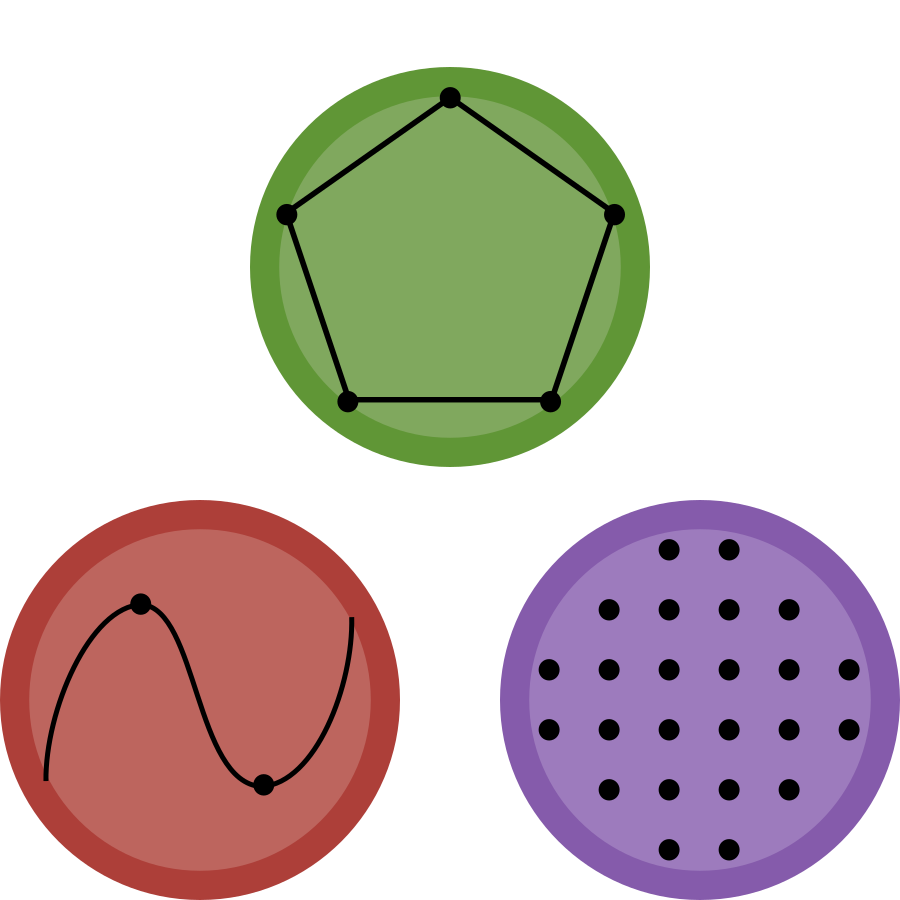
\includegraphics[scale=0.04]{../../latex/images/juliaopt.png}};
          \node at (4,-1.65) {JuliaOpt};
          \SetVertexNormal[Shape=rectangle,FillColor = red!50]
          \Vertex[x=3,y=0,L={\jlpkg{SwitchedSystems}*}]{SS}
          \SetVertexNormal[Shape=rectangle,FillColor = blue!30]
          \Vertex[x=0,y=-1.1,L={\jlpkg{PolyJuMP}*${}^{(1)}$}]{PJMP}
          \Vertex[x=3,y=-2.3,L={\jlpkg{JuMP}}]{JMP}
          \Vertex[x=0,y=-2.5,L={\jlpkg{SumOfSquares}*${}^{(1)}$}]{SOS}
          \SetVertexNormal[Shape=rectangle,FillColor = green!50]
          \Vertex[x=-3,y=0,L={\jlpkg{MultivariatePolynomials}*${}^{(1)}$}]{MP}
          \Vertex[x=3,y=-3,L={\jlpkg{MathProgBase}}]{MPB}
          \SetVertexNormal[Shape=rectangle,FillColor = yellow!50]
          \Vertex[x=0,y=-3.5,L={\jlpkg{Mosek}}]{Mosek}
          \Vertex[x=1,y=-4,L={\jlpkg{SCS}}]{SCS}
          \Vertex[x=3,y=-4,L={\jlpkg{CSDP}*${}^{(2)}$}]{CSDP}
          \Vertex[x=4,y=-3.5,L={\jlpkg{SDPA}*}]{SDPA}
          \tikzset{EdgeStyle/.style={->}}
          \Edge(SS)(PJMP)
          \Edge(PJMP)(MP)
          \Edge(PJMP)(SOS)
          \Edge(PJMP)(JMP)
          \Edge(SOS)(MP)
          \Edge(JMP)(MPB)
          \Edge(MPB)(Mosek)
          \Edge(MPB)(SCS)
          \Edge(MPB)(CSDP)
          \Edge(MPB)(SDPA)
          \node at (-4,-2.5) {
            \begin{minipage}{3.2cm}
              \begin{itemize}
                \item \alert{Separate} Julia packages.
                \item Can be used \alert{independently}.
              \end{itemize}
            \end{minipage}
          };
          \node[right] at (-5.8,-4.2) {\tiny * New};
          \node[right] at (-5.8,-4.4) {\tiny ${}^{(1)}$ Joint work with Robin Deits, Joey Huchette, Chris Coey and Amelia Perry of MIT};
          \node[right] at (-5.8,-4.6) {\tiny ${}^{(2)}$ Joint work with Elias Kuthe of Universit\"at Duisburg Essen};
        \end{tikzpicture}
      \end{center}
  \end{frame}
  \begin{frame}{Conclusion}
    \begin{block}{Results}
      \begin{itemize}
        \item Lower bound \alert{certificate} using measures.
        \item Detection of \alert{atomic} measures and extraction of \alert{periodic} trajectory.
        \item Algorithm for producing \alert{guaranteed} high-growth sequences.
        \item Guarantee depending on \alert{topology} of the automaton.
        \item \alert{Convex} program provides both upper and lower bounds.
      \end{itemize}
    \end{block}
    \begin{block}{Open questions}
      \begin{itemize}
        \item Improved \alert{guarantees}? What is best possible?
        \item Is the sequence always \alert{periodic} for a fixed $d$ ? Can we bound the period ?
      \end{itemize}
    \end{block}
  \end{frame}

  \begin{frame}{Why is it a relaxation ?}
  \Wider{
      The Semidefinite Programming constraints on the trunctated moments of $\mu_\sigma$ are necessary for the existence of a measure with those moments,
  and \alert{any} value of the moments of higher degree (not necessarily 0).

  In the Common Quadratic Lyapunov Function case, i.e. $2d = 2$, those conditions are necessary and sufficient.
  \begin{itemize}
      \item For every truncated moments, we can find a $\mu_\sigma$ that has these moments.
      \item And there exists a slack variable $\mu_{\mathrm{slack}}$ such that
          \[ \sum_{\sigma=1}^m \Exp_{\mu_\sigma}[p(A_\sigma x)] - \gamlb^{2d} \sum_{\sigma = 1}^m \Exp_{\mu_\sigma}[p(x)] = \Exp_{\mu_{\mathrm{slack}}}, \forall p(x) \in \Sosh, \]
          so
          \[ \sum_{\sigma=1}^m \mathcal{A}_\sigma \mu_\sigma - \gamlb^{2d} \sum_{\sigma = 1}^m \mu_\sigma \only<1>{=}\only<2>{\text{ has the same trunctated moments than }} \mu_{\mathrm{slack}} \]
  \end{itemize}
  }
\end{frame}

  \begin{frame}{Adjacency matrix}
  \Wider{\cssystemtikz{40}{20}%
    \uncover<2->{\[ \rho(\Adj) = \lim_{k \to \infty} \norm{\Adj^k}^{1/k}. \]}%
  \begin{minipage}{0.35\textwidth}
    \begin{align*}
      \only<1-3>{
        \Adj & =
        \begin{pmatrix}
          0 & 1 & 1 & 0\\
          1 & 0 & 1 & 0\\
          1 & 1 & 1 & 1\\
          0 & 0 & 1 & 0
        \end{pmatrix}.
      }
      \only<4>{
        \Adj^2 & =
        \begin{pmatrix}
          2 & 1 & 2 & 1\\
          1 & 2 & 2 & 1\\
          2 & 2 & 4 & 1\\
          1 & 1 & 1 & 1
        \end{pmatrix}.
      }
      \only<5>{
        \Adj^3 & =
        \begin{pmatrix}
          3 & 4 & 6 & 2\\
          4 & 3 & 6 & 2\\
          6 & 6 & 9 & 4\\
          2 & 2 & 4 & 1
        \end{pmatrix}.
      }
    \end{align*}
  \end{minipage}
  \begin{minipage}{0.6\textwidth}
    \begin{align*}
      \only<3>{
        \norm{\Adj}_\infty & = \max
        \begin{pmatrix}
          0 + 1 + 1 + 0\\
          1 + 0 + 1 + 0\\
          1 + 1 + 1 + 1\\
          0 + 0 + 1 + 0
        \end{pmatrix} =
        \begin{pmatrix}
          2\\2\\4\\1
        \end{pmatrix}.%
      }
      \only<4>{
        \norm{\Adj^2}_\infty & = \max
        \begin{pmatrix}
          2 + 1 + 2 + 1\\
          1 + 2 + 2 + 1\\
          2 + 2 + 4 + 1\\
          1 + 1 + 1 + 1
        \end{pmatrix} =
        \begin{pmatrix}
          6\\6\\9\\4
        \end{pmatrix}.%
      }
      \only<5>{
        \norm{\Adj^3}_\infty & = \max
        \begin{pmatrix}
          3 + 4 + 6 + 2\\
          4 + 3 + 6 + 2\\
          6 + 6 + 9 + 4\\
          2 + 2 + 4 + 1
        \end{pmatrix} =
        \begin{pmatrix}
          15\\15\\25\\9
        \end{pmatrix}.
      }
    \end{align*}
\end{minipage}}
\end{frame}

\end{document}
